\begin{filecontents}{pictexa.tex}
\documentclass{article}
\usepackage{epic,eepic,pspicture,mathptmx,times,graphpap}
\begin{document}
\pagestyle{empty}
\begin{picture}(60,40)(-2,-2)
\setlength{\unitlength}{1mm}
%\graphpaper(0,0)(70,50)
\arrowlength{2mm}\linethickness{1pt}
\put(0,0){\Vector(60,0)}
\put(0,0){\Vector(0,40)}
\thicklines
\put(15,0){\Line(35,35)}
\thinlines
\dashline{3}(50,0)(50,35)
\dashline{3}(0,35)(50,35)
\dashline{2}(15,0)(15,35)
\put(15,0){\arc{19}{4.7124}{5.4978}}
\put(17.5,10.5){\ensuremath{\displaystyle\theta}}
\put(1,37){\emph{h}}
\put(51,2){\emph{n(h)}}
\end{picture}
\end{document}
\end{filecontents}
\begin{filecontents*}{pictexa.eps}
%!PS-Adobe-2.0 EPSF-2.0
%%Creator: dvips(k) 5.94b Copyright 2004 Radical Eye Software
%%Title: pictexa.dvi
%%BoundingBox: 148 627 322 745
%%DocumentFonts: Symbol Times-Italic
%%EndComments
%DVIPSWebPage: (www.radicaleye.com)
%DVIPSCommandLine: dvips -E pictexa -opictexa.eps
%DVIPSParameters: dpi=600, compressed
%DVIPSSource:  TeX output 2005.05.30:1757
%%BeginProcSet: texc.pro 0 0
%!
/TeXDict 300 dict def TeXDict begin/N{def}def/B{bind def}N/S{exch}N/X{S
N}B/A{dup}B/TR{translate}N/isls false N/vsize 11 72 mul N/hsize 8.5 72
mul N/landplus90{false}def/@rigin{isls{[0 landplus90{1 -1}{-1 1}ifelse 0
0 0]concat}if 72 Resolution div 72 VResolution div neg scale isls{
landplus90{VResolution 72 div vsize mul 0 exch}{Resolution -72 div hsize
mul 0}ifelse TR}if Resolution VResolution vsize -72 div 1 add mul TR[
matrix currentmatrix{A A round sub abs 0.00001 lt{round}if}forall round
exch round exch]setmatrix}N/@landscape{/isls true N}B/@manualfeed{
statusdict/manualfeed true put}B/@copies{/#copies X}B/FMat[1 0 0 -1 0 0]
N/FBB[0 0 0 0]N/nn 0 N/IEn 0 N/ctr 0 N/df-tail{/nn 8 dict N nn begin
/FontType 3 N/FontMatrix fntrx N/FontBBox FBB N string/base X array
/BitMaps X/BuildChar{CharBuilder}N/Encoding IEn N end A{/foo setfont}2
array copy cvx N load 0 nn put/ctr 0 N[}B/sf 0 N/df{/sf 1 N/fntrx FMat N
df-tail}B/dfs{div/sf X/fntrx[sf 0 0 sf neg 0 0]N df-tail}B/E{pop nn A
definefont setfont}B/Cw{Cd A length 5 sub get}B/Ch{Cd A length 4 sub get
}B/Cx{128 Cd A length 3 sub get sub}B/Cy{Cd A length 2 sub get 127 sub}
B/Cdx{Cd A length 1 sub get}B/Ci{Cd A type/stringtype ne{ctr get/ctr ctr
1 add N}if}B/id 0 N/rw 0 N/rc 0 N/gp 0 N/cp 0 N/G 0 N/CharBuilder{save 3
1 roll S A/base get 2 index get S/BitMaps get S get/Cd X pop/ctr 0 N Cdx
0 Cx Cy Ch sub Cx Cw add Cy setcachedevice Cw Ch true[1 0 0 -1 -.1 Cx
sub Cy .1 sub]/id Ci N/rw Cw 7 add 8 idiv string N/rc 0 N/gp 0 N/cp 0 N{
rc 0 ne{rc 1 sub/rc X rw}{G}ifelse}imagemask restore}B/G{{id gp get/gp
gp 1 add N A 18 mod S 18 idiv pl S get exec}loop}B/adv{cp add/cp X}B
/chg{rw cp id gp 4 index getinterval putinterval A gp add/gp X adv}B/nd{
/cp 0 N rw exit}B/lsh{rw cp 2 copy get A 0 eq{pop 1}{A 255 eq{pop 254}{
A A add 255 and S 1 and or}ifelse}ifelse put 1 adv}B/rsh{rw cp 2 copy
get A 0 eq{pop 128}{A 255 eq{pop 127}{A 2 idiv S 128 and or}ifelse}
ifelse put 1 adv}B/clr{rw cp 2 index string putinterval adv}B/set{rw cp
fillstr 0 4 index getinterval putinterval adv}B/fillstr 18 string 0 1 17
{2 copy 255 put pop}for N/pl[{adv 1 chg}{adv 1 chg nd}{1 add chg}{1 add
chg nd}{adv lsh}{adv lsh nd}{adv rsh}{adv rsh nd}{1 add adv}{/rc X nd}{
1 add set}{1 add clr}{adv 2 chg}{adv 2 chg nd}{pop nd}]A{bind pop}
forall N/D{/cc X A type/stringtype ne{]}if nn/base get cc ctr put nn
/BitMaps get S ctr S sf 1 ne{A A length 1 sub A 2 index S get sf div put
}if put/ctr ctr 1 add N}B/I{cc 1 add D}B/bop{userdict/bop-hook known{
bop-hook}if/SI save N @rigin 0 0 moveto/V matrix currentmatrix A 1 get A
mul exch 0 get A mul add .99 lt{/QV}{/RV}ifelse load def pop pop}N/eop{
SI restore userdict/eop-hook known{eop-hook}if showpage}N/@start{
userdict/start-hook known{start-hook}if pop/VResolution X/Resolution X
1000 div/DVImag X/IEn 256 array N 2 string 0 1 255{IEn S A 360 add 36 4
index cvrs cvn put}for pop 65781.76 div/vsize X 65781.76 div/hsize X}N
/p{show}N/RMat[1 0 0 -1 0 0]N/BDot 260 string N/Rx 0 N/Ry 0 N/V{}B/RV/v{
/Ry X/Rx X V}B statusdict begin/product where{pop false[(Display)(NeXT)
(LaserWriter 16/600)]{A length product length le{A length product exch 0
exch getinterval eq{pop true exit}if}{pop}ifelse}forall}{false}ifelse
end{{gsave TR -.1 .1 TR 1 1 scale Rx Ry false RMat{BDot}imagemask
grestore}}{{gsave TR -.1 .1 TR Rx Ry scale 1 1 false RMat{BDot}
imagemask grestore}}ifelse B/QV{gsave newpath transform round exch round
exch itransform moveto Rx 0 rlineto 0 Ry neg rlineto Rx neg 0 rlineto
fill grestore}B/a{moveto}B/delta 0 N/tail{A/delta X 0 rmoveto}B/M{S p
delta add tail}B/b{S p tail}B/c{-4 M}B/d{-3 M}B/e{-2 M}B/f{-1 M}B/g{0 M}
B/h{1 M}B/i{2 M}B/j{3 M}B/k{4 M}B/w{0 rmoveto}B/l{p -4 w}B/m{p -3 w}B/n{
p -2 w}B/o{p -1 w}B/q{p 1 w}B/r{p 2 w}B/s{p 3 w}B/t{p 4 w}B/x{0 S
rmoveto}B/y{3 2 roll p a}B/bos{/SS save N}B/eos{SS restore}B end

%%EndProcSet
%%BeginProcSet: pspicture.ps 0 0
%!
%%
%% Source File `pspicture.dtx'.
%% Copyright (C) 1992 1999 David Carlisle
%% This file may be distributed under the terms of the LPPL.
%% See 00readme.txt for details.
%%




/!BP{
  72 72.27 div dup scale
  }def
/!A{
  newpath
  0 0 moveto
  dup neg dup .4 mul rlineto
  .8 mul 0 exch  rlineto
  closepath
  fill
  } def
/!V{
  !BP
  /!X exch def
  /!y exch def
  /!x exch def
  newpath
  0 0 moveto
  !x 0 eq {0  !y 0 lt {!X neg}{!X} ifelse}
         {!x 0 lt {!X neg}{!X}ifelse  !X !y mul !x abs div} ifelse
  lineto
  setlinewidth  % @wholewidth
  currentpoint
  stroke
  translate
  !y !x atan
  rotate
  !A            % @arrowlength
  }def
/!L{
  !BP
  /!X exch def
  /!y exch def
  /!x exch def
  newpath
  0 0 moveto
  !x 0 eq {0  !y 0 lt {!X neg}{!X} ifelse}
         {!x 0 lt {!X neg}{!X}ifelse  !X !y mul !x abs div} ifelse
  lineto
  setlinewidth  % @wholewidth
  stroke
  }def
/!C{
  !BP
  0 0 3 2 roll
  2 div 0 360 arc
  setlinewidth  % @wholewidth
  stroke
  }def
/!D{
  !BP
  0 0 3 2 roll
  2 div 0 360 arc fill
  }def
/!O{
  !BP
  /!y exch 2 div def
  /!x exch 2 div def
  /!r exch !x !y
    2 copy gt {exch} if pop
    2 copy gt {exch} if pop
      def
  setlinewidth  % @wholewidth
  1 eq
  {newpath
   !x neg 0 moveto
   !x neg !y 0 !y !r arcto 4 {pop} repeat
   0 !y lineto
   stroke}if
  1 eq
  {newpath
   !x  0 moveto
   !x  !y 0 !y !r arcto 4 {pop} repeat
   0 !y lineto
   stroke}if
  1 eq
  {newpath
   !x neg 0 moveto
   !x neg !y neg 0 !y neg  !r arcto 4 {pop} repeat
   0 !y neg lineto
   stroke}if
  1 eq
  {newpath
   !x  0 moveto
   !x  !y neg 0 !y neg !r arcto 4 {pop} repeat
   0 !y neg lineto
   stroke}if
  }def
/!V2{
  !BP
  2 copy exch
  atan
  /a exch def
  2 copy
  newpath
  0 0 moveto
  lineto          % <x*unitlength> <y*unitlength>
  3 2 roll
  setlinewidth  % @wholewidth
  stroke
  translate       % <x*unitlength> <y*unitlength>
  a rotate
  !A                    % @arrowlength
  }def
/!L2{
  !BP
  newpath
  0 0 moveto
  lineto          % <x*unitlength> <y*unitlength>
  setlinewidth  % @wholewidth
  stroke
  }def
/!C2{
  !BP
  /!s exch def
  /!y exch def
  /!x exch def
  newpath
  0 0 moveto
  0 0
  !x 2 div !y 10 div !s mul add
  !y 2 div  !x 10 div  !s mul sub
  !x !y
  curveto
  setlinewidth  % @wholewidth
  stroke
  }def

%%EndProcSet
%%BeginProcSet: 8r.enc 0 0
% @@psencodingfile@{
%   author    = "S. Rahtz, P. MacKay, Alan Jeffrey, B. Horn, K. Berry,
%                W. Schmidt, P. Lehman",
%   version   = "20021105.19",
%   date      = "5 November 2002",
%   filename  = "8r.enc",
%   email     = "tex-fonts@@tug.org",
%   docstring = "This is the encoding vector for Type1 and TrueType
%                fonts to be used with TeX.  This file is also included
%                in the PSNFSS bundle."
% @}
% 
% The idea is to have all the characters normally included in Type 1 fonts
% available for typesetting. This is effectively the characters in Adobe
% Standard encoding, ISO Latin 1, Windows ANSI including the euro symbol,
% MacRoman, and some extra characters from Lucida.
% 
% Character code assignments were made as follows:
% 
% (1) the Windows ANSI characters are almost all in their Windows ANSI
% positions, because some Windows users cannot easily reencode the
% fonts, and it makes no difference on other systems. The only Windows
% ANSI characters not available are those that make no sense for
% typesetting -- rubout (127 decimal), nobreakspace (160), softhyphen
% (173). quotesingle and grave are moved just because it's such an
% irritation not having them in TeX positions.
% 
% (2) Remaining characters are assigned arbitrarily to the lower part
% of the range, avoiding 0, 10 and 13 in case we meet dumb software.
% 
% (3) Y&Y Lucida Bright includes some extra text characters; in the
% hopes that other PostScript fonts, perhaps created for public
% consumption, will include them, they are included starting at 0x12.
% These are /dotlessj /ff /ffi /ffl.
% 
% (4) hyphen appears twice for compatibility with both ASCII and Windows.
%
% (5) /Euro was assigned to 128, as in Windows ANSI.
%
% (6) Missing characters from MacRoman encoding incorporated in October
% 2002 as follows:
%
%     PostScript      MacRoman        TeXBase1
%     --------------  --------------  --------------
%     /notequal       173             0x16
%     /infinity       176             0x17
%     /lessequal      178             0x18
%     /greaterequal   179             0x19
%     /partialdiff    182             0x1A
%     /summation      183             0x1B
%     /product        184             0x1C
%     /pi             185             0x1D
%     /integral       186             0x81
%     /Omega          189             0x8D
%     /radical        195             0x8E
%     /approxequal    197             0x8F
%     /Delta          198             0x9D
%     /lozenge        215             0x9E
%
/TeXBase1Encoding [
% 0x00
 /.notdef /dotaccent /fi /fl
 /fraction /hungarumlaut /Lslash /lslash
 /ogonek /ring /.notdef /breve
 /minus /.notdef /Zcaron /zcaron
% 0x10
 /caron /dotlessi /dotlessj /ff
 /ffi /ffl /notequal /infinity
 /lessequal /greaterequal /partialdiff /summation
 /product /pi /grave /quotesingle
% 0x20
 /space /exclam /quotedbl /numbersign
 /dollar /percent /ampersand /quoteright
 /parenleft /parenright /asterisk /plus
 /comma /hyphen /period /slash
% 0x30
 /zero /one /two /three
 /four /five /six /seven
 /eight /nine /colon /semicolon
 /less /equal /greater /question
% 0x40
 /at /A /B /C
 /D /E /F /G
 /H /I /J /K
 /L /M /N /O
% 0x50
 /P /Q /R /S
 /T /U /V /W
 /X /Y /Z /bracketleft
 /backslash /bracketright /asciicircum /underscore
% 0x60
 /quoteleft /a /b /c
 /d /e /f /g
 /h /i /j /k
 /l /m /n /o
% 0x70
 /p /q /r /s
 /t /u /v /w
 /x /y /z /braceleft
 /bar /braceright /asciitilde /.notdef
% 0x80
 /Euro /integral /quotesinglbase /florin
 /quotedblbase /ellipsis /dagger /daggerdbl
 /circumflex /perthousand /Scaron /guilsinglleft
 /OE /Omega /radical /approxequal
% 0x90
 /.notdef /.notdef /.notdef /quotedblleft
 /quotedblright /bullet /endash /emdash
 /tilde /trademark /scaron /guilsinglright
 /oe /Delta /lozenge /Ydieresis
% 0xA0
 /.notdef /exclamdown /cent /sterling
 /currency /yen /brokenbar /section
 /dieresis /copyright /ordfeminine /guillemotleft
 /logicalnot /hyphen /registered /macron
% 0xD0
 /degree /plusminus /twosuperior /threesuperior
 /acute /mu /paragraph /periodcentered
 /cedilla /onesuperior /ordmasculine /guillemotright
 /onequarter /onehalf /threequarters /questiondown
% 0xC0
 /Agrave /Aacute /Acircumflex /Atilde
 /Adieresis /Aring /AE /Ccedilla
 /Egrave /Eacute /Ecircumflex /Edieresis
 /Igrave /Iacute /Icircumflex /Idieresis
% 0xD0
 /Eth /Ntilde /Ograve /Oacute
 /Ocircumflex /Otilde /Odieresis /multiply
 /Oslash /Ugrave /Uacute /Ucircumflex
 /Udieresis /Yacute /Thorn /germandbls
% 0xE0
 /agrave /aacute /acircumflex /atilde
 /adieresis /aring /ae /ccedilla
 /egrave /eacute /ecircumflex /edieresis
 /igrave /iacute /icircumflex /idieresis
% 0xF0
 /eth /ntilde /ograve /oacute
 /ocircumflex /otilde /odieresis /divide
 /oslash /ugrave /uacute /ucircumflex
 /udieresis /yacute /thorn /ydieresis
] def

%%EndProcSet
%%BeginProcSet: texps.pro 0 0
%!
TeXDict begin/rf{findfont dup length 1 add dict begin{1 index/FID ne 2
index/UniqueID ne and{def}{pop pop}ifelse}forall[1 index 0 6 -1 roll
exec 0 exch 5 -1 roll VResolution Resolution div mul neg 0 0]FontType 0
ne{/Metrics exch def dict begin Encoding{exch dup type/integertype ne{
pop pop 1 sub dup 0 le{pop}{[}ifelse}{FontMatrix 0 get div Metrics 0 get
div def}ifelse}forall Metrics/Metrics currentdict end def}{{1 index type
/nametype eq{exit}if exch pop}loop}ifelse[2 index currentdict end
definefont 3 -1 roll makefont/setfont cvx]cvx def}def/ObliqueSlant{dup
sin S cos div neg}B/SlantFont{4 index mul add}def/ExtendFont{3 -1 roll
mul exch}def/ReEncodeFont{CharStrings rcheck{/Encoding false def dup[
exch{dup CharStrings exch known not{pop/.notdef/Encoding true def}if}
forall Encoding{]exch pop}{cleartomark}ifelse}if/Encoding exch def}def
end

%%EndProcSet
%%BeginProcSet: special.pro 0 0
%!
TeXDict begin/SDict 200 dict N SDict begin/@SpecialDefaults{/hs 612 N
/vs 792 N/ho 0 N/vo 0 N/hsc 1 N/vsc 1 N/ang 0 N/CLIP 0 N/rwiSeen false N
/rhiSeen false N/letter{}N/note{}N/a4{}N/legal{}N}B/@scaleunit 100 N
/@hscale{@scaleunit div/hsc X}B/@vscale{@scaleunit div/vsc X}B/@hsize{
/hs X/CLIP 1 N}B/@vsize{/vs X/CLIP 1 N}B/@clip{/CLIP 2 N}B/@hoffset{/ho
X}B/@voffset{/vo X}B/@angle{/ang X}B/@rwi{10 div/rwi X/rwiSeen true N}B
/@rhi{10 div/rhi X/rhiSeen true N}B/@llx{/llx X}B/@lly{/lly X}B/@urx{
/urx X}B/@ury{/ury X}B/magscale true def end/@MacSetUp{userdict/md known
{userdict/md get type/dicttype eq{userdict begin md length 10 add md
maxlength ge{/md md dup length 20 add dict copy def}if end md begin
/letter{}N/note{}N/legal{}N/od{txpose 1 0 mtx defaultmatrix dtransform S
atan/pa X newpath clippath mark{transform{itransform moveto}}{transform{
itransform lineto}}{6 -2 roll transform 6 -2 roll transform 6 -2 roll
transform{itransform 6 2 roll itransform 6 2 roll itransform 6 2 roll
curveto}}{{closepath}}pathforall newpath counttomark array astore/gc xdf
pop ct 39 0 put 10 fz 0 fs 2 F/|______Courier fnt invertflag{PaintBlack}
if}N/txpose{pxs pys scale ppr aload pop por{noflips{pop S neg S TR pop 1
-1 scale}if xflip yflip and{pop S neg S TR 180 rotate 1 -1 scale ppr 3
get ppr 1 get neg sub neg ppr 2 get ppr 0 get neg sub neg TR}if xflip
yflip not and{pop S neg S TR pop 180 rotate ppr 3 get ppr 1 get neg sub
neg 0 TR}if yflip xflip not and{ppr 1 get neg ppr 0 get neg TR}if}{
noflips{TR pop pop 270 rotate 1 -1 scale}if xflip yflip and{TR pop pop
90 rotate 1 -1 scale ppr 3 get ppr 1 get neg sub neg ppr 2 get ppr 0 get
neg sub neg TR}if xflip yflip not and{TR pop pop 90 rotate ppr 3 get ppr
1 get neg sub neg 0 TR}if yflip xflip not and{TR pop pop 270 rotate ppr
2 get ppr 0 get neg sub neg 0 S TR}if}ifelse scaleby96{ppr aload pop 4
-1 roll add 2 div 3 1 roll add 2 div 2 copy TR .96 dup scale neg S neg S
TR}if}N/cp{pop pop showpage pm restore}N end}if}if}N/normalscale{
Resolution 72 div VResolution 72 div neg scale magscale{DVImag dup scale
}if 0 setgray}N/psfts{S 65781.76 div N}N/startTexFig{/psf$SavedState
save N userdict maxlength dict begin/magscale true def normalscale
currentpoint TR/psf$ury psfts/psf$urx psfts/psf$lly psfts/psf$llx psfts
/psf$y psfts/psf$x psfts currentpoint/psf$cy X/psf$cx X/psf$sx psf$x
psf$urx psf$llx sub div N/psf$sy psf$y psf$ury psf$lly sub div N psf$sx
psf$sy scale psf$cx psf$sx div psf$llx sub psf$cy psf$sy div psf$ury sub
TR/showpage{}N/erasepage{}N/setpagedevice{pop}N/copypage{}N/p 3 def
@MacSetUp}N/doclip{psf$llx psf$lly psf$urx psf$ury currentpoint 6 2 roll
newpath 4 copy 4 2 roll moveto 6 -1 roll S lineto S lineto S lineto
closepath clip newpath moveto}N/endTexFig{end psf$SavedState restore}N
/@beginspecial{SDict begin/SpecialSave save N gsave normalscale
currentpoint TR @SpecialDefaults count/ocount X/dcount countdictstack N}
N/@setspecial{CLIP 1 eq{newpath 0 0 moveto hs 0 rlineto 0 vs rlineto hs
neg 0 rlineto closepath clip}if ho vo TR hsc vsc scale ang rotate
rwiSeen{rwi urx llx sub div rhiSeen{rhi ury lly sub div}{dup}ifelse
scale llx neg lly neg TR}{rhiSeen{rhi ury lly sub div dup scale llx neg
lly neg TR}if}ifelse CLIP 2 eq{newpath llx lly moveto urx lly lineto urx
ury lineto llx ury lineto closepath clip}if/showpage{}N/erasepage{}N
/setpagedevice{pop}N/copypage{}N newpath}N/@endspecial{count ocount sub{
pop}repeat countdictstack dcount sub{end}repeat grestore SpecialSave
restore end}N/@defspecial{SDict begin}N/@fedspecial{end}B/li{lineto}B
/rl{rlineto}B/rc{rcurveto}B/np{/SaveX currentpoint/SaveY X N 1
setlinecap newpath}N/st{stroke SaveX SaveY moveto}N/fil{fill SaveX SaveY
moveto}N/ellipse{/endangle X/startangle X/yrad X/xrad X/savematrix
matrix currentmatrix N TR xrad yrad scale 0 0 1 startangle endangle arc
savematrix setmatrix}N end

%%EndProcSet
TeXDict begin 40258437 52099154 1000 600 600 (pictexa.dvi)
@start /Fa 145[42 5[42 62[28 28 40[{TeXBase1Encoding ReEncodeFont}4
83.022 /Times-Italic rf /Fb 142[43 113[{.167 SlantFont}1
83.022 /Symbol rf end
%%EndProlog
%%BeginSetup
%%Feature: *Resolution 600dpi
TeXDict begin
 end
%%EndSetup
TeXDict begin 1 0 bop 656 756 a @beginspecial @setspecial
5.69054 1.0 170.71564 0.0 !V2


@endspecial @beginspecial @setspecial
5.69054 1.0 0.0 113.81042 !V2
 
@endspecial 354
w @beginspecial @setspecial
0.79999 99.58412 99.58412 !L2
 
@endspecial 3 setlinewidth
np 1837 756 a 1837 687 li st 3 setlinewidth np 1837 604
a 1837 535 li st 3 setlinewidth np 1837 452 a 1837 383
li st 3 setlinewidth np 1837 301 a 1837 232 li st 3 setlinewidth
np 1837 149 a 1837 80 li st 3 setlinewidth np 1837 -2
a 1837 -71 li st 3 setlinewidth np 656 -71 a 725 -71
li st 3 setlinewidth np 815 -71 a 884 -71 li st 3 setlinewidth
np 973 -71 a 1042 -71 li st 3 setlinewidth np 1132 -71
a 1201 -71 li st 3 setlinewidth np 1291 -71 a 1360 -71
li st 3 setlinewidth np 1450 -71 a 1519 -71 li st 3 setlinewidth
np 1609 -71 a 1678 -71 li st 3 setlinewidth np 1767 -71
a 1836 -71 li st 3 setlinewidth np 1010 756 a 1010 713
li st 3 setlinewidth np 1010 658 a 1010 615 li st 3 setlinewidth
np 1010 560 a 1010 517 li st 3 setlinewidth np 1010 462
a 1010 419 li st 3 setlinewidth np 1010 364 a 1010 321
li st 3 setlinewidth np 1010 266 a 1010 223 li st 3 setlinewidth
np 1010 168 a 1010 125 li st 3 setlinewidth np 1010 70
a 1010 27 li st 3 setlinewidth np 1010 -28 a 1010 -71
li st 3 setlinewidth np 1010 756 224 270.00 315.00 arc
st 1069 507 a Fb(q)679 -119 y Fa(h)1861 708 y(n\(h\))p
eop end
%%Trailer

userdict /end-hook known{end-hook}if
%%EOF
\end{filecontents*}
\documentclass{cernrep}
\begin{document}
\title{Title of contribution}
\author{A.N. Author and A.N. Other\thanks
                 {On leave from another institue somewhere.}}
\institute{Institute name in English, Town, Country}
\maketitle

\begin{abstract}
Each paper should be preceded by a short abstract of not more 
than 150~words, which should be written as a single paragraph 
and should not contain references.
\end{abstract}

\section{Section heading}

A section title is styled as above, and first paragraphs after
headings are not indented. References appear in numerical
order~\cite{Raby1966,Dupont1961}. An itemized list looks like the following:
\begin{itemize}
\item the first item,
\item the second item.
\end{itemize}

You can also have an enumerated list:

\begin{enumerate}
\item the first item,
\item the second item.
\end{enumerate}

\subsection{Subsection heading}

As you see the first paragraph is not indented. References when part
      of the text use the term `Ref.', for example, see
      Ref.~\cite{Raby1966} and
      Refs.~\cite{Appleman1959,vanBerg1965,Bryant1985,Allen1977}.

Subsequent paragraphs are indented. See Table~\ref{tab:LET} for an
example of how to display a table.

\begin{table}[h]
\begin{center}
\caption{A simple table}
\label{tab:LET}
\begin{tabular}{p{6cm}cc}
\hline\hline
\textbf{Heading}             & \textbf{Result 1}
                                                & \textbf{Result 2}\\
\hline
200 kVp X-rays total$^{a}$   & 3.25             & 1.79 \\
200 kVp X-rays (primary)     & 2.60             & 1.48 \\
\hline\hline
\multicolumn{3}{l}{$^{a}$ \footnotesize Notes in tables appear as
                      this one here.}
\end{tabular}
\end{center}
\end{table}

\subsubsection{Subsubsection title}
\label{sec:sss}

Equation~(\ref{eq:a1}) is presented correctly:
\begin{equation}
n^k(h)= k h \frac{k}{32}~. \label{eq:a1}  
\end{equation}

This is how all equations should be formatted,
including~Eqs.~(2)--(10), 
%% With LaTeX use: Eqs,~(\ref{eq:a2})--(\ref{eq:a10}) syntax.
which are not shown\footnote{Footnotes are
to be used only when absolutely necessary.}.

\subsubsubsection{Subsubsubsection title}

Figure~\ref{tab:LET} is an example of how to display figures. Please
refer to figures as Figs.~2--4, etc.
%% With LaTeX use : Figs.~\ref{fig:a1}--\ref{fig:a4} syntax.
Section~\ref{sec:sss} is a cross-reference to a section. 
See the document describing the CERN reports~\cite{cernrep} for more
details on how to present figures, tables, equations, and much more
with \LaTeX. 

\begin{figure}[ht]
\begin{center}
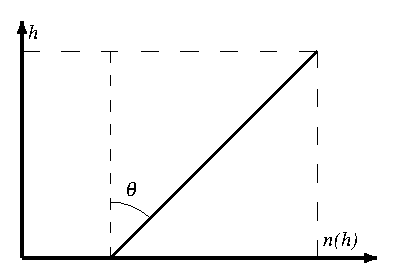
\includegraphics[width=6cm]{pictexa}
\caption{Diagram of a straight line}
\label{fig:line}
\end{center}
\end{figure}

Examples of references and a bibliography follow the acknowledgements.

\section*{Acknowledgements}

We wish to thank A.N. Colleague for enlightening comments on
the present topic.

\begin{thebibliography}{99}
\bibitem{Raby1966}
J.M. Raby, Biophysical aspects of radiation quality, International 
Atomic EnergyAgency, Technical Reports Series No. 58 (1966).
\bibitem{Dupont1961}
J.-P. Dupont, Proc. Int. Conf. on Radiation Hazards, Columbia, 
1960 (Academic Press Inc., New York, 1961), Vol. II, p. 396.
\bibitem{Appleman1959}
H. Appleman \emph{et al.}, J. \emph{Med. Biol.} \textbf{8} (1959) 911.
\bibitem{vanBerg1965}
E. van Berg, D. Johnson and J. Smith, \emph{Rad. Res.} \textbf{5} (1965) 
215.
\bibitem{Bryant1985}
P. Bryant and S. Newman (Eds.), The generation of high fields, 
CAS--ECFA--INFN Workshop, Frascati, 1984., ECFA 85/91, CERN 85/07 
(1985).
\bibitem{Allen1977}
M.A. Allen \emph{et al.}, \emph{IEEE Trans. Nucl. Sci.} \textbf{NS--24} (1977) 
1780.
\bibitem{cernrep}
DTP Section, Preparing contributions to CERN reports,
\url{http://cern.ch/DTP/cernrep.pdf}.
\end{thebibliography}

\section*{Bibliography}


I.C. Percival and D. Richards, \emph{Introduction to Dynamics}
(Cambridge University Press, Cambridge, 1982).

\appendix
\section{Title of appendix}
\label{sec:app}

\subsection{Subsection title in appendix}

Inside an appendix the same level of headings (section, subsection,
etc.) as in the main text applies. Only the first number is replaced
by an uppercase letter.

\subsubsection{Subsubsection title in appendix}

Inside a subsubsection inside an appendix.

\subsubsubsection{Subsubsubsection title in appendix}

\end{document}
